\documentclass{article}
\usepackage{graphicx} % Required for inserting images
\usepackage[margin=2.5cm]{geometry}
\usepackage{amsmath, amssymb}
\usepackage{setspace}
\usepackage{float}
\usepackage{hyperref}

\title{NLP assignment 1: Theoretical Answers}
\author{Dan Ben-David, Elad Erdman}
\date{November 2026}

\begin{document}
\maketitle

\section*{Question 2: Implementing word2vec}

\subsection*{Part e - Training results}

\begin{figure}[ht]
    \centering
    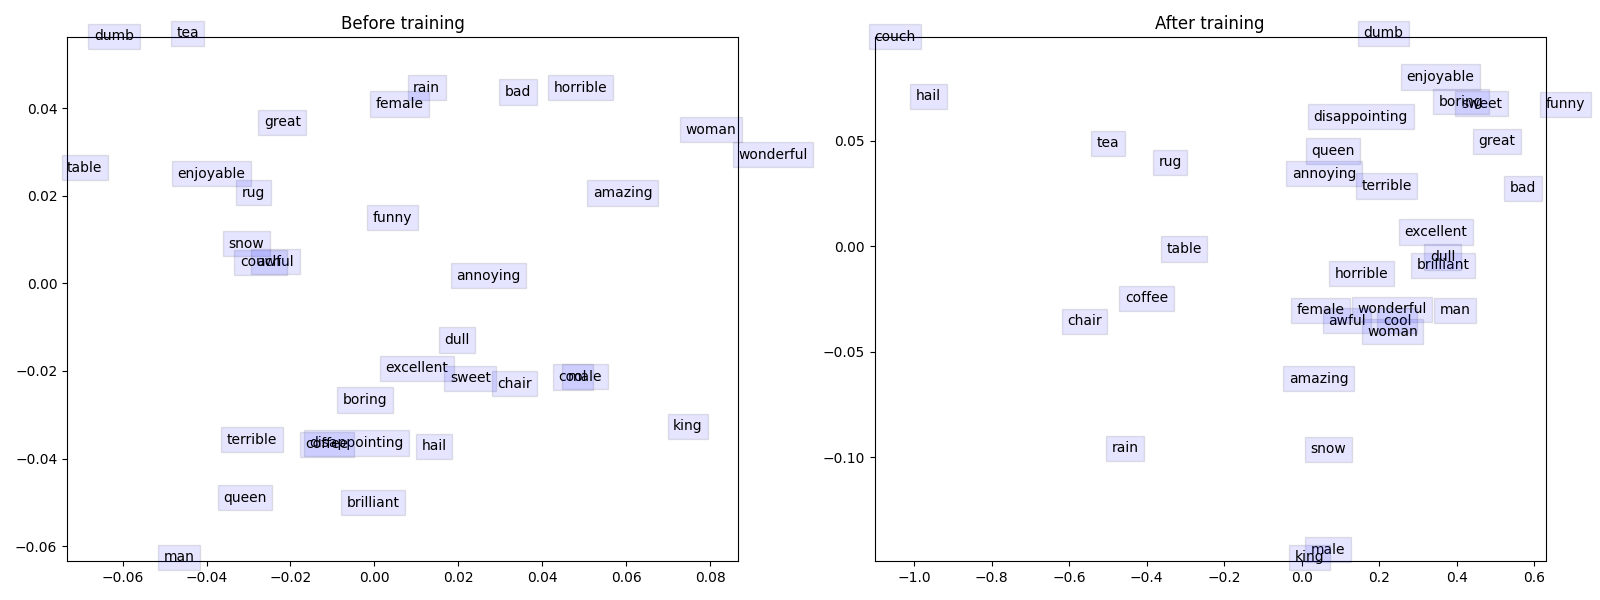
\includegraphics[width=1.0\textwidth]{word_vectors.png}
    \label{Training picture results}
\end{figure}


\subsection*{Part f - Results discussion}

\subsubsection*{1)}
The plot demonstrates that the model successfully clustered words with similar semantic roles. For example, many adjectives are grouped in the top right, nouns are clustered in the middle left, and weather-related terms are grouped at the bottom.

\subsubsection*{2)}
The word vectors perform as expected regarding basic semantic grouping, but they fail to capture sentiment, clustering positive and negative adjectives, for example "great" and "bad", "excellent" and "horrible", are closely together . This happens because word2vec model relies on context window and positive and negative adjective will probably be near the same words. To improve the vectors we could train the model with larger dimensions to capture those nuances or modify it to explicitly incorporate sentiment weights.

\clearpage
\section*{Question 3: Optimizing word2vec}

\subsection*{(a)}
    $$J(\theta) = \sum_{t=1}^T \sum_{-m \le j \le m, j \ne 0}\log p_\theta(w_{t+j}|w_t)$$
The sum in the objective function counts how many times the outer word is near the center word so instead we can count on every pair of center and outside words times \#(c,o) by definition, and we get:
    $$J(\theta) = \sum_{c \in V} \sum_{o \in V}\#(c,o)\log p_{\theta}(o|c)$$
We must enforce the constraint that for every $c \in V$ $\sum_{o \in V} p(o|c) = 1$\\
The Lagrangian for a specific center word c is
\begin{gather*}
    L_c = \sum_{o \in V} \#(c,o)\log p(o|c) -\lambda \left(\sum_{o \in V} p(o|c)-1\right) \\
    \frac {\partial L_c}{\partial p(o \mid c)} = \frac{\#(c,o)}{p(o \mid c)} - \lambda = 0 \text{ (compare to 0 for maximum)} \\ 
    p(o|c)=\frac{\#(c,o)}{\lambda}
\end{gather*}
The sum of full distribution ends up to be 1 thus
    $$1=\sum_{o} p(o \mid c)=\sum_{o} \frac{\#(c,o)}{\lambda}\quad\longrightarrow\quad\lambda = \sum_{o}\#(c,o)$$
Substituting $\lambda$ back, we get the optimal distribution
    $$p_{\theta^*}(o \mid c) = \frac{\#(c,o)}{\sum_{o'} \#(c,o')}$$

\subsection*{(b)}
We will use the same example given in the question, but focus on b as a center word instead.\\
It is easy to see that $p(b|b) = 0$. But we can see in the example:
    $$p(a|a) = \frac{2}{3}, \quad p(b|a) = \frac{2}{9}$$
then we get
    $$\frac{p(a|a)}{p(b|a)} = 3$$
On the other hand
\begin{gather*}
    3 = \frac{p(a|a)}{p(b|a)} = \frac{e^{u_a \cdot v_a}}{e^{u_b \cdot v_a}} = e^{(u_a - u_b)v_a}\\
    \ln (3) = (u_a - u_b)v_a
\end{gather*}
This results in $u_a \ne u_b$ and they are real numbers. But when we check 'b' as a center word, we get:
\begin{itemize}
    \setlength{\itemsep}{0pt}
    \item $p(a|b) = 1$
    \item $p(b|b) = 0$
    \item $p(c|b) = 0$
\end{itemize}
because only 'a' occurs next to 'b'. However, then we get:
\begin{gather*}
    0 = p(b\vert{}b) = \frac{e^{u_b \cdot v_b}}{\sum_o e^{u_o \cdot v_b}}
\end{gather*}
Since the denominator is finite and positive, for the fraction to be zero, the numerator must be zero:
\begin{gather*}
    0 = e^{u_b \cdot v_b} = e^{\text{real number}} > 0
\end{gather*}
This results in a mathematical contradiction because $e^x > 0$ for every real number $x$.\\
Thus, no real-valued parameters can satisfy this condition, proving that the scalar Skip-gram model is fundamentally incapable of reaching the optimal empirical distribution in this case.


\clearpage
\section*{AI disclosure and reflection}

\subsection*{Google Gemini 1.5 Flash}

The model was used for checking the correct syntax for commands for NumPy library and shortcuts in LaTeX, for faster search instead of online guidelines. Used in Question 2 for NumPy and LaTeX in Question 3.\\
Reflection: The model helped me quickly and accurately understand how to use relevant commands.\\



\end{document}
